\section{Auswertung}
\label{sec:Auswertung}

\subsection{Darstellung der Moden}
Die Reflektorspannungen $U$, die Spannungsamplituden $A$, sowie Frequenzen $f$ für drei verschiedene Moden sind in Tabelle 1 dargestellt.
Die Stromstärke beträgt dabei $I = 25$mA.



\begin{table}[H]
  \centering
  \caption{Reflektorspannungen, die Spannungsamplituden und die Frequenzen der drei Moden}
  \label{tab:Parameter}
  \begin{tabular}{c c c c}
    \toprule
    Mode & $U/$V & $A/$mV& $f/\left(\frac{1}{s}\right)$\\
    \midrule
    1. & 83  &   119,9& 8999 \\
       & 95  & &       \\
       & 105 & &       \\
    2. & 135 &    152,4 & 8994 \\
       & 150 & & \\
       & 165 & & \\
    3. & 215 &  139,7  & 8988 \\
       & 230 & & \\
       & 245 & & \\
    \bottomrule
  \end{tabular}
\end{table}

Durch die drei Punkte kann eine Anpassungsfunktion gelegt werden der Form:
\begin{equation*}
  f(x)=ax^2+bx+c
\end{equation*}

Dies ist in Abbildung 6 dargestellt.
\begin{figure}
  \centering
  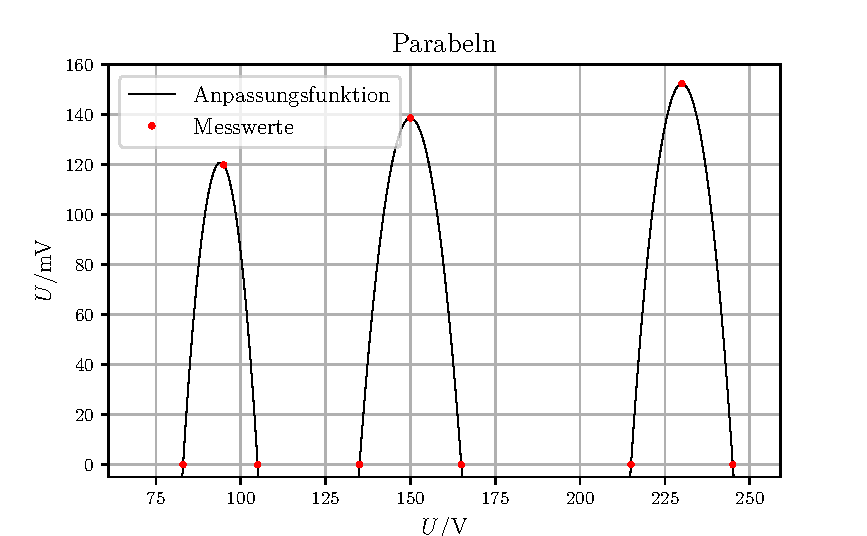
\includegraphics{plot1.pdf}
  \caption{Anpassungsfunktionen für die Messwerte der drei Moden}
  \label{fig:plot}
\end{figure}



\subsection{Frequenz, Wellenlänge und Dämpfung}
Die Abstände der Minima zu dem jeweiligen nächsten Minima betragen $\SI{113.0}{\milli\meter}$, $\SI{90.0}{\milli\meter}$,
$\SI{65.0}{\milli\meter}$ und $\SI{42.0}{\milli\meter}$.
Für den Mittelwert der Wellenlänge im Hohlleiter ergibt sich $\lambda_{\symup{g}} =\SI{4.73(13)}{\centi\meter}$.
Der Fehler wird dabei mit der gaußschen Fehlerfortpflanzung von Python \cite{uncertainties} bestimmt.

Da bei den Mikrowellen im Hohlleiter $TE_{1,0}$-Moden vorliegen, kann die Frequenz der
Mikrowellen im freien Raum mit Gleichung (4), sowie die Wellenlänge im freien Raum mit Gleichung (1)
bestimmt werden.

\begin{align*}
  f &= \SI{9.10(12)}{\giga\hertz} \\
  \lambda_{0} &= \SI{33.0(4)}{\milli\meter}
\end{align*}

Dabei beträgt die Breitseite des Hohlleiters $a= \SI{23.0}{\milli\meter}$.
Die kritische Wellenlänge $\lambda_{\symup{c}}$ wird mit Gleichung (3) berechnet.
\begin{equation*}
  \lambda_{\symup{c}} = 2a = \SI{4.6}{\centi\meter}
\end{equation*}

Die Phasengeschwindigkeit der Mikrowelle im Hohlleiter ist:
\begin{align*}
  &v_{\symup{ph}} = f \cdot \lambda_{\symup{g}} = \SI{4.30(13)e11}{\milli\meter\per\second} \\
\text{mit}\:\:  &\lambda_{\symup{g}} =\SI{47.3(13)}{\milli\meter}
\end{align*}

Die Dämpfung $D$, in Abhängigkeit von der Tiefe $d$ der Mikrometerschraube des Abschwächers, ist in Tabelle 2
dargestellt. Dabei sind einmal die gemessenen Werte der Dämpfung $D_1$, sowie die Dämpfungswerte der
Eichkurve $D_2$ angegeben.


\begin{table}[H]
  \centering
  \caption{Dämpfungen in Abhängigkeit von der Tiefe der Mikrometerschraube}
  \label{tab:Parameter}
  \begin{tabular}{c c c}
    \toprule
    $d$/mm & $D_1/$dB & $D_2/$dB\\
    \midrule
    1,0 &  0  & 2,1    \\
    1,7 &  0,2  & 5,9    \\
    2,0 &  0,6  & 7,9    \\
    2,5 &  2,7  & 11,0    \\
    2,8 &  4,9  & 14,0    \\
    2,9 &  6,0  & 15,0    \\
    3,0 &  6,8  & 16,0    \\
    3,1 &  8,1  & 18,0    \\
    3,2 &  8,9  & 19,0    \\
    3,3 &  10,0 & 20,0    \\
    \bottomrule
  \end{tabular}
\end{table}

In Abbildung 7 sind die Messwerte in einem Diagramm dargestellt.

\begin{figure}
  \centering
  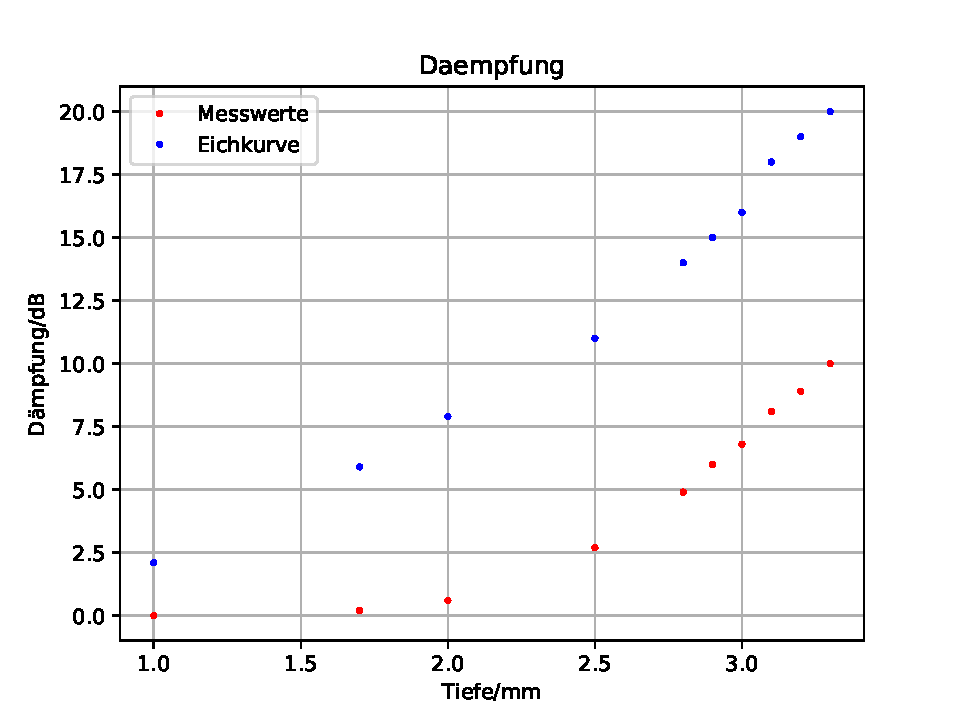
\includegraphics{daempfung.pdf}
  \caption{Eichkurve und gemessene Dämpfungen}
  \label{fig:plot}
\end{figure}

\subsection{Bestimmung des Welligkeitsverhältnisses}
\subsubsection{Direkte Methode}
Bei der direkten Methode wird das Welligkeitsverhältnis (Stehwellenverhältnis) direkt
vom SWR-Meter abgelesen. Die entsprechenden Werte sind in Tabelle \ref{tab:direkt} zu finden.

\begin{table}[H]
  \centering
  \caption{Stehwellenverhältnis in Abhängigkeit der Stifttiefe des Gleitschraubentransformators bei der direkten Methode}
  \label{tab:direkt}
  \begin{tabular}{c c}
    \toprule
    $d$/mm & SWR \\
    \midrule
    0 &  1,02    \\
    3 &  1,17    \\
    5 &  1,47    \\
    7 &  2,30    \\
    \bottomrule
  \end{tabular}
\end{table}

\subsubsection{3dB Methode}
Die gemessenen Abstände nach links und rechts, die sich bei der 3dB-Methode ergeben haben,
lauten
\begin{align*}
  d_\symup{l} &= 83\, \symup{mm} \\
  d_\symup{r} &= 71\, \symup{mm}
\end{align*}

Die Stifttiefe beträgt dabei $9\, \symup{mm}$.
Daraus ergibt sich nach Gleichung (6) das Welligkeitsverhältnis:

\begin{equation*}
  S = 1,719 \pm 0,024
\end{equation*}

Dabei wird für die Wellenlänge im Hohlleiter das oben bereits genannte Ergebnis von $\lambda_g = 4,73 \pm 0,13 \, \symup{cm}$ verwendet.

\subsubsection{Abschwächermethode}
Die Dämpfung vor bzw. nachdem das Maximum des Ausgangssignals dem Minimum
gleichgemacht wird, werden gemessen zu
\begin{align*}
  A_\symup{vor} &= 20 \, \symup{dB} \\
  A_\symup{nach} &= 38,5 \, \symup{dB}
\end{align*}

Damit lässt sich nach Gleichung (8) das SWR berechnen:
\begin{equation*}
  S = 10^{\frac{A_\symup{nach}-A_\symup{vor}}{20}} = 8,414
\end{equation*}
